% Supplementary sections set aside on 2026-11-20 at the user's request (the supplement keeps the ablation and
% inpainting sections). Not input by main.tex; content and numbers are kept for later use.
% The protocol, provenance, objectives, judging, human review, valid-cell text and tab:supp_isr_full are
% now in X_suppl.tex (sections C and D); the copies here are not maintained.

\section{Protocol details}
\label{sec:supp_protocol}
\paragraph{Data.} We select the portraits from the metadata of a public collection of 9{,}853 Pexels portraits in which every image contains a detected face, and download each image at a width of 1200 pixels. The selection consists of six steps. (1)~We keep images whose description contains words for exactly one of man and woman and none of a list of exclusion words (children, groups, black-and-white, occlusion, artistic rendering), which leaves 5{,}763 images. (2)~We require that MTCNN detects exactly one face with probability at least 0.98, that the face height is 0.07 to 0.50 of the shorter image side, that the face is near-frontal (horizontal offset of the nose tip at most 0.25 of the inter-eye distance), that the image is not grayscale (mean $|a^*| + |b^*| \ge 6$ in CIELAB), and that the face box lies inside the crop, which leaves 2{,}486 images. (3)~We require that the zero-shot gender probability of CLIP ViT-L/14 is at least 0.8 and agrees with the description, and that FaceNet returns an identity embedding, which leaves 2{,}459 images (407 men and 2{,}052 women). (4)~We rank the images by CLIP image similarity to eight reference portraits, keep at most two images per photographer, and treat pairs with FaceNet identity cosine similarity of at least 0.65 as the same person. (5)~We remove images with occlusion, profile views, closed eyes, small subjects, face paint, children, nudity, or underexposure by visual inspection. (6)~We remove six images whose subject mask covers less than 1\% or more than 80\% of the image or misses the person. The gender ratio of the resulting set follows the number of men that pass step~(3). We record the Pexels identifier, photographer, description, original size, face box, crop box, and checksum of each image. We crop each portrait to a square of side $\min(H, W)$ centered $0.18$ side lengths below the center of the detected face box, clamp the square to the image, and resize it to $512\times512$ with Lanczos resampling. We obtain subject masks with CLIPSeg (\texttt{CIDAS/clipseg-rd64-refined}, the class name as text prompt, threshold 0.30, dilation by 4 pixels); the masks define the inpainting region in \cref{sec:supp_inpainting} and are not used by any defense.

\paragraph{Editors.} For cross-model transferability, we use VIBE-DistilledCFG (\texttt{iitolstykh/VIBE-Image-Edit-DistilledCFG}, revision a10edb9, 20 sampling steps, other settings at the pipeline defaults) and the distilled FLUX.2 [klein] 4B (\texttt{black-forest-labs/FLUX.2-klein-4B}, revision e7b7dc2, bf16, 4 steps, guidance 1.0) at $512\times512$ with seed 20260812; both receive the instructions in the form ``Add sunglasses to the person''. The undefended edit of each image and instruction uses the same seed as the immunized edit, so that the two differ only in the input image. All editors receive the immunized images obtained against InstructPix2Pix, without re-optimization. The inpainting editor (\texttt{runwayml/stable-diffusion-inpainting}, revision 8a4288a, fp32) is described in \cref{sec:supp_inpainting}.

\paragraph{Purifications.} Cropping removes 10\% from each side and resizes the result to $512\times512$ with bicubic interpolation; rotation uses bilinear interpolation and zero fill. Each purification is applied to the immunized image, and the edit of the purified image is compared with the edit of the original image under the same purification. VAE-Trans reconstructs the immunized image through a VAE whose encoder is fine-tuned on clean images.

\paragraph{VAE-Trans.} We reproduce VAE-Trans~\cite{purifyonce2026} on the VAE of InstructPix2Pix (\texttt{timbrooks/instruct-pix2pix}, revision 31519b5). Only the encoder and the quantization convolution are fine-tuned; the decoder is frozen. The input is $x + \eta$ with $\eta \sim \mathcal{N}(0, 0.1^2)$ on the $[0, 1]$ scale, and the target is the posterior mean of the frozen original encoder for the clean image $x$, with a mean squared error loss. Following the paper, we use AdamW with learning rate $10^{-4}$ for 6 epochs; the batch size of 2 and random $512\times512$ crops are our choices, as the paper does not state them. Training uses 2{,}000 OmniEdit images, validation 64, and seed 0; the validation latent error decreases from 16.99 to 3.33. At inference, the purified image is the decoding of the posterior mean of the fine-tuned encoder, without sampling, at $512\times512$.

\paragraph{Matched-distortion rescaling.} We first run each additive defense at the budget of its paper (\cref{tab:supp_provenance}). To approximately match perceptual distortion, we multiply the budget $\epsilon$ by a factor chosen on a calibration set of 8 portraits so that the mean defense LPIPS equals 0.3344, the value of an earlier color-based variant, and apply the factors unchanged to the 306 portraits. We scale the step size by the same factor so that the ratio of step size to budget is unchanged, and keep all other settings. The rescaled settings therefore differ from those of the original papers; for DCT-Shield and DCT-Shield-Y, the rescaled budget falls below one quantization level, so the condition under which these papers state robustness to JPEG compression no longer holds. LPIPS is computed with \texttt{piq.LPIPS} (VGG) on the delivered 8-bit images.

\section{Baseline provenance and budget conversion}
\label{sec:supp_provenance}
\Cref{tab:supp_provenance} lists the native settings of each additive defense, the factor applied to its budget in the matched-distortion setting, and the source of the implementation. We port the official code where it is available and otherwise reimplement the method from the description in its paper.

\begin{table*}[t]
  \centering
  \footnotesize
  \setlength{\tabcolsep}{5pt}
  \caption{Native settings of the additive methods, the factor applied to $\epsilon$ in the matched-distortion arm, and the source of the implementation. Budgets are on the $[0, 1]$ pixel scale unless stated. Official: the authors' code, ported to this pipeline (commit in parentheses); Reimpl.: reimplemented from the paper. $^{a}$The code path enabled in the official notebook; the paper (Table~9) states an $L_\infty$ budget of 16/255 with step 2/255. $^{b}$Budget on the DCT coefficients with sign updates, step size $\eta_i = (1 - i/N)\,\gamma$ at step $i$ of $N$ with $\gamma = 0.1$, $Q_{\mathrm{alg}} = 0.95$ (0.85 for DCT-Shield-Y, luminance only); reimplemented from Algorithm~1 of the paper's supplement; in the matched-distortion arm, $\gamma$ is scaled by the same factor as $\epsilon$. $^{c}$Learning rate; $\sigma$-weighting 10. In the matched-distortion arm the $\sigma$-weighting is 0 and the solved perturbation is multiplied by 0.6071. $^{d}$Official code; the commit is not recorded. $^{e}$The paper states $\epsilon = 0.06$ and the step $2/255$ on the $[-1, 1]$ scale.}
  \label{tab:supp_provenance}
  \begin{tabular}{@{}l l l c l c l@{}}
    \toprule
    Method & Budget $\epsilon$ & Step size & Steps & Norm & $\epsilon$ factor & Source \\
    \midrule
    PhotoGuard (encoder)~\cite{salman2023photoguard} & 0.03$^{a}$ & 0.01$^{a}$ & 1000 & $L_\infty$, sign PGD & 0.2614 & Official (686bea7) \\
    Mist~\cite{liang2023mist} & 16/255 & 1/255 & 100 & $L_\infty$ & 0.125 & Official (99f5f3c) \\
    DIA-PT~\cite{dia2025} & 6.4/255 & 1/255 & 20 & $L_\infty$ & 0.418 & Official$^{d}$ \\
    DIA-R~\cite{dia2025} & 6.4/255 & 1/255 & 20 & $L_\infty$ & 0.969 & Official$^{d}$ \\
    DCT-Shield~\cite{dctshield2025} & 1$^{b}$ & $\gamma$, linearly decayed$^{b}$ & 1000 & DCT, sign$^{b}$ & 0.211 & Reimpl. \\
    DCT-Shield-Y~\cite{dctshield2025} & 1$^{b}$ & $\gamma$, linearly decayed$^{b}$ & 1000 & DCT, Y only, sign$^{b}$ & 0.073 & Reimpl. \\
    SIFM~\cite{dong2025sifm} & 7.65/255 & 1/255 (not stated) & 100 & $L_\infty$ & 0.289 & Reimpl. \\
    DAYN~\cite{lo2024dayn} & 0.03$^{e}$ & 1/255 (not stated)$^{e}$ & 100 & $L_\infty$ & 0.43 & Reimpl. \\
    DANP~\cite{zhang2025danp} & 0.03 & 1/255 (not stated) & 100 & $L_\infty$ & 0.323 & Reimpl. \\
    BlurGuard~\cite{blurguard2025} & 16/255 & 0.06$^{c}$ & 150 & $L_\infty$ & 0.6071$^{c}$ & Official (e1b2d5e) \\
    \bottomrule
  \end{tabular}
\end{table*}

\paragraph{Objectives.} PhotoGuard maximizes the $\ell_2$ norm of the posterior mean of the VAE encoder, without text conditioning. Mist combines a textual loss with the fixed target text ``a painting'' and a semantic loss (fused mode~2). DIA-PT maximizes the $\ell_2$ distance between the latent obtained by the diffusion and inversion process and the encoder latent; DIA-R maximizes the $\ell_2$ distance in pixel space between the reconstruction from this latent and the immunized image. DCT-Shield maximizes the $\ell_2$ norm of the encoder latent without text conditioning. SIFM uses a mean squared error on the mid-block output of the SD~v1.4 U-Net at $t \in \{200, 400, 600, 800\}$. DAYN disperses the cross-attention maps (Eq.~5 of the paper), with the subject mask applied to the attention maps; DANP combines the DAA and NBA objectives (Eqs.~11--13 of the paper); both use the class name as text condition and average the gradient over 10 repetitions. BlurGuard uses the frequency-weighted PGD of the official code. All solvers use seed 0.

\section{Additional metrics}
\label{sec:supp_metrics}
\Cref{tab:supp_aesthetics} reports additional quality measures of the immunized images, and \cref{tab:supp_edit_metrics} reports the edit-level metrics that are not listed in \cref{tab:main}, averaged over the seven image purifications. \Cref{tab:supp_purification_first,tab:supp_purification_second} provide the edit displacement under each purification, of which \cref{tab:main} reports the mean over the seven purifications.

\begin{table*}[t]
  \begin{minipage}[t]{0.44\textwidth}
  \centering
  \footnotesize
  \setlength{\tabcolsep}{4pt}
  \caption{Additional measurements of the immunized images (306 Pexels portraits, matched-distortion arms): PSNR and SSIM against the original image, and the no-reference scores NIMA and NIQE. LPIPS, LAION, and MUSIQ are in \cref{tab:main}. Best in bold.}
  \label{tab:supp_aesthetics}
  \begin{tabular}{l cc cc}
    \toprule
    & \multicolumn{2}{c}{vs.\ original} & \multicolumn{2}{c}{No-reference} \\
    \cmidrule(lr){2-3} \cmidrule(l){4-5}
    Method & PSNR $\uparrow$ & SSIM $\uparrow$ & NIMA $\uparrow$ & NIQE $\downarrow$ \\
    \midrule
    \textcolor{gray}{Original} & \textcolor{gray}{--} & \textcolor{gray}{--} & \textcolor{gray}{5.399} & \textcolor{gray}{4.061} \\
    \midrule
    DAYN & 40.6 & .981 & 5.208 & 4.135 \\
    DIA-R & 40.3 & .981 & 5.283 & 4.049 \\
    DIA-PT & 42.5 & .988 & 5.265 & 3.867 \\
    SIFM & \textbf{43.2} & .989 & 5.300 & 3.995 \\
    DANP & 43.0 & .988 & 5.286 & 3.993 \\
    Mist & 43.1 & \textbf{.991} & 5.339 & 3.997 \\
    PhotoGuard & 42.7 & .990 & 5.315 & 4.083 \\
    DCT-Shield & 39.3 & .980 & \textbf{5.380} & 4.823 \\
    DCT-Shield-Y & 37.7 & .987 & 5.351 & 4.633 \\
    BlurGuard & 38.1 & .946 & 5.083 & \textbf{3.420} \\
    \midrule
    \rowcolor{oursrow}
    \textbf{\capg{}} & 24.2 & .928 & 5.278 & 3.979 \\
    \bottomrule
  \end{tabular}
  \end{minipage}\hfill
  \begin{minipage}[t]{0.52\textwidth}
  \centering
  \footnotesize
  \setlength{\tabcolsep}{3pt}
  \caption{Edit-level metrics not listed in \cref{tab:main} (306 Pexels portraits $\times$ 4 instructions, InstructPix2Pix, matched-distortion arms), each the mean over the seven image purifications. SSIM, PSNR, and CLIP-I compare the immunized and the undefended edit under the same purification; CLIP-S compares the immunized edit with the instruction text; FID and KID are computed between the sets of immunized and undefended edits. Per-purification values are in \cref{tab:supp_purification_first,tab:supp_purification_second}. Best in bold.}
  \label{tab:supp_edit_metrics}
  \begin{tabular}{@{}l cccccc@{}}
    \toprule
    Method & SSIM $\downarrow$ & PSNR $\downarrow$ & CLIP-I $\downarrow$ & CLIP-S $\downarrow$ & FID $\uparrow$ & KID$\times10^3$ $\uparrow$ \\
    \midrule
    DAYN & .900 & 28.2 & .949 & .241 & 26.1 & 2.15 \\
    DIA-R & .908 & 28.6 & .957 & .239 & 23.7 & 1.21 \\
    DIA-PT & .918 & 29.4 & .960 & .238 & 24.4 & 2.04 \\
    SIFM & .921 & 29.6 & .964 & .242 & 21.0 & 0.48 \\
    DANP & .916 & 29.3 & .964 & .242 & 21.5 & 0.59 \\
    Mist & .924 & 30.2 & .968 & .238 & 20.7 & 1.05 \\
    PhotoGuard & .923 & 30.2 & .969 & .239 & 21.4 & 1.44 \\
    DCT-Shield & .940 & 31.6 & .975 & .240 & 17.9 & 0.60 \\
    DCT-Shield-Y & .939 & 31.3 & .980 & .241 & 17.4 & 0.10 \\
    BlurGuard & .855 & 26.7 & .936 & \textbf{.233} & 38.9 & \textbf{8.94} \\
    \midrule
    \rowcolor{oursrow}
    \textbf{\capg{}} & \textbf{.807} & \textbf{19.0} & \textbf{.889} & .235 & \textbf{44.7} & 7.44 \\
    \bottomrule
  \end{tabular}
  \end{minipage}
\end{table*}

% Generated by docs/paper_tools/generate_per_purification_table.py; do not edit by hand.
\begin{table*}[t]
  \centering
  \footnotesize
  \setlength{\tabcolsep}{4pt}
  \begin{tabular}{l ccccccc c}
    \toprule
    Method & JPEG 80 & JPEG 50 & JPEG 30 & Blur $\sigma{=}1$ & Blur $\sigma{=}2$ & Crop & Rotation & VAE-Trans \\
    \midrule
    \multicolumn{9}{l}{\textit{Edit LPIPS $\uparrow$}} \\
    DAYN & .246 & .214 & .190 & .178 & .106 & .303 & .246 & .056 \\
    DIA-R & .242 & .203 & .180 & .173 & .094 & .282 & .234 & .051 \\
    DIA-PT & .218 & .181 & .162 & .161 & .078 & .279 & .223 & .041 \\
    SIFM & .201 & .171 & .148 & .137 & .070 & .259 & .206 & .036 \\
    DANP & .210 & .178 & .153 & .148 & .077 & .275 & .218 & .041 \\
    Mist & .172 & .148 & .142 & .120 & .063 & .294 & .209 & .033 \\
    PhotoGuard & .166 & .146 & .137 & .114 & .056 & .282 & .199 & .033 \\
    DCT-Shield & .095 & .099 & .096 & .062 & .028 & .254 & .154 & .023 \\
    DCT-Shield-Y & .118 & .113 & .122 & .051 & .035 & .223 & .136 & .029 \\
    BlurGuard & .300 & .282 & .275 & .280 & .208 & .298 & .279 & .143 \\
    \rowcolor{oursrow}
    \textbf{\capg{}} & .372 & .386 & .401 & .357 & .360 & .355 & .317 & .288 \\
    \midrule
    \multicolumn{9}{l}{\textit{SSIM between the two edits $\downarrow$}} \\
    DAYN & .879 & .892 & .900 & .928 & .964 & .858 & .881 & .970 \\
    DIA-R & .885 & .898 & .904 & .936 & .970 & .871 & .889 & .971 \\
    DIA-PT & .902 & .911 & .913 & .945 & .975 & .883 & .899 & .977 \\
    SIFM & .902 & .915 & .921 & .947 & .976 & .881 & .901 & .980 \\
    DANP & .896 & .909 & .918 & .944 & .975 & .874 & .894 & .978 \\
    Mist & .918 & .926 & .925 & .958 & .981 & .865 & .898 & .982 \\
    PhotoGuard & .921 & .927 & .927 & .959 & .982 & .850 & .895 & .982 \\
    DCT-Shield & .947 & .947 & .948 & .974 & .989 & .864 & .912 & .987 \\
    DCT-Shield-Y & .935 & .938 & .932 & .978 & .987 & .880 & .925 & .983 \\
    BlurGuard & .832 & .838 & .839 & .872 & .923 & .839 & .843 & .942 \\
    \rowcolor{oursrow}
    \textbf{\capg{}} & .806 & .797 & .789 & .819 & .832 & .798 & .812 & .858 \\
    \midrule
    \multicolumn{9}{l}{\textit{PSNR between the two edits (dB) $\downarrow$}} \\
    DAYN & 26.1 & 27.4 & 28.0 & 29.8 & 33.9 & 25.4 & 26.6 & 31.3 \\
    DIA-R & 26.5 & 27.6 & 28.2 & 30.4 & 34.8 & 25.9 & 26.8 & 31.4 \\
    DIA-PT & 27.4 & 28.4 & 28.7 & 31.3 & 36.1 & 26.4 & 27.4 & 32.6 \\
    SIFM & 27.3 & 28.6 & 29.1 & 31.6 & 36.7 & 26.2 & 27.7 & 33.4 \\
    DANP & 27.0 & 28.2 & 29.0 & 31.4 & 36.4 & 26.0 & 27.3 & 32.8 \\
    Mist & 28.5 & 29.3 & 29.4 & 33.3 & 38.1 & 25.5 & 27.5 & 33.9 \\
    PhotoGuard & 28.6 & 29.4 & 29.5 & 33.5 & 38.5 & 24.5 & 27.2 & 34.1 \\
    DCT-Shield & 30.3 & 30.6 & 30.7 & 35.4 & 40.6 & 25.3 & 28.2 & 35.5 \\
    DCT-Shield-Y & 29.3 & 29.9 & 29.4 & 36.2 & 39.5 & 25.8 & 28.9 & 34.1 \\
    BlurGuard & 25.7 & 26.1 & 26.3 & 27.2 & 29.9 & 25.8 & 25.9 & 28.8 \\
    \rowcolor{oursrow}
    \textbf{\capg{}} & 18.9 & 18.9 & 19.0 & 19.0 & 19.1 & 18.8 & 19.3 & 19.7 \\
    \midrule
    \multicolumn{9}{l}{\textit{SigLIP $\downarrow$}} \\
    DAYN & .937 & .952 & .963 & .954 & .971 & .923 & .937 & .986 \\
    DIA-R & .947 & .959 & .967 & .962 & .977 & .940 & .947 & .988 \\
    DIA-PT & .951 & .962 & .971 & .963 & .980 & .939 & .946 & .990 \\
    SIFM & .959 & .968 & .975 & .970 & .984 & .943 & .954 & .992 \\
    DANP & .959 & .965 & .973 & .971 & .983 & .943 & .954 & .990 \\
    Mist & .968 & .976 & .976 & .978 & .988 & .929 & .951 & .992 \\
    PhotoGuard & .969 & .976 & .975 & .979 & .988 & .925 & .951 & .992 \\
    DCT-Shield & .984 & .983 & .982 & .987 & .993 & .931 & .960 & .994 \\
    DCT-Shield-Y & .980 & .980 & .979 & .990 & .991 & .944 & .968 & .993 \\
    BlurGuard & .930 & .937 & .939 & .934 & .948 & .930 & .928 & .970 \\
    \rowcolor{oursrow}
    \textbf{\capg{}} & .888 & .888 & .888 & .882 & .878 & .882 & .890 & .901 \\
    \bottomrule
  \end{tabular}
  \caption{Edit displacement for each purification (first part; 306 Pexels portraits $\times$ 4 instructions, InstructPix2Pix, matched-distortion arms). Each entry is the mean over the 306 images, each image first averaged over the four instructions; \cref{tab:main} reports the mean over the seven purifications. SSIM, PSNR, SigLIP, CLIP-I, and ArcFace compare the defended and the undefended edit under the same purification; CLIP-S compares the defended edit with the instruction text; FID is computed between the sets of defended and undefended edits.}
  \label{tab:supp_purification_first}
\end{table*}

\begin{table*}[t]
  \centering
  \footnotesize
  \setlength{\tabcolsep}{4pt}
  \begin{tabular}{l ccccccc c}
    \toprule
    Method & JPEG 80 & JPEG 50 & JPEG 30 & Blur $\sigma{=}1$ & Blur $\sigma{=}2$ & Crop & Rotation & VAE-Trans \\
    \midrule
    \multicolumn{9}{l}{\textit{CLIP-I $\downarrow$}} \\
    DAYN & .938 & .953 & .966 & .953 & .974 & .922 & .940 & .988 \\
    DIA-R & .944 & .958 & .969 & .959 & .980 & .938 & .948 & .990 \\
    DIA-PT & .950 & .967 & .976 & .959 & .983 & .938 & .946 & .992 \\
    SIFM & .955 & .969 & .978 & .967 & .986 & .941 & .955 & .993 \\
    DANP & .957 & .968 & .978 & .969 & .985 & .941 & .954 & .992 \\
    Mist & .970 & .979 & .980 & .979 & .991 & .929 & .952 & .994 \\
    PhotoGuard & .973 & .979 & .980 & .980 & .991 & .927 & .952 & .994 \\
    DCT-Shield & .988 & .986 & .985 & .985 & .995 & .932 & .955 & .996 \\
    DCT-Shield-Y & .983 & .984 & .983 & .993 & .994 & .950 & .973 & .994 \\
    BlurGuard & .929 & .937 & .944 & .933 & .955 & .930 & .928 & .972 \\
    \rowcolor{oursrow}
    \textbf{\capg{}} & .883 & .886 & .890 & .889 & .895 & .883 & .896 & .894 \\
    \midrule
    \multicolumn{9}{l}{\textit{CLIP-S $\downarrow$}} \\
    DAYN & .243 & .242 & .240 & .241 & .245 & .240 & .237 & .245 \\
    DIA-R & .238 & .240 & .239 & .238 & .244 & .238 & .236 & .245 \\
    DIA-PT & .237 & .239 & .238 & .239 & .245 & .236 & .234 & .244 \\
    SIFM & .242 & .242 & .239 & .241 & .245 & .242 & .239 & .246 \\
    DANP & .242 & .242 & .240 & .241 & .246 & .242 & .241 & .246 \\
    Mist & .239 & .241 & .239 & .238 & .244 & .232 & .235 & .245 \\
    PhotoGuard & .240 & .241 & .239 & .239 & .245 & .233 & .236 & .245 \\
    DCT-Shield & .242 & .242 & .240 & .240 & .245 & .233 & .236 & .245 \\
    DCT-Shield-Y & .243 & .242 & .241 & .241 & .246 & .235 & .238 & .246 \\
    BlurGuard & .233 & .233 & .233 & .232 & .240 & .232 & .230 & .242 \\
    \rowcolor{oursrow}
    \textbf{\capg{}} & .236 & .236 & .234 & .235 & .238 & .236 & .232 & .242 \\
    \midrule
    \multicolumn{9}{l}{\textit{ArcFace $\downarrow$}} \\
    DAYN & .825 & .849 & .859 & .906 & .950 & .847 & .851 & .943 \\
    DIA-R & .837 & .859 & .860 & .911 & .958 & .864 & .863 & .941 \\
    DIA-PT & .851 & .873 & .874 & .923 & .963 & .864 & .856 & .951 \\
    SIFM & .855 & .883 & .888 & .931 & .967 & .861 & .873 & .961 \\
    DANP & .844 & .872 & .884 & .929 & .963 & .856 & .861 & .957 \\
    Mist & .890 & .895 & .890 & .947 & .969 & .868 & .879 & .965 \\
    PhotoGuard & .895 & .900 & .898 & .949 & .971 & .866 & .890 & .968 \\
    DCT-Shield & .922 & .922 & .919 & .963 & .979 & .881 & .906 & .974 \\
    DCT-Shield-Y & .903 & .914 & .893 & .965 & .975 & .883 & .906 & .966 \\
    BlurGuard & .846 & .835 & .822 & .871 & .916 & .882 & .858 & .913 \\
    \rowcolor{oursrow}
    \textbf{\capg{}} & .784 & .760 & .750 & .806 & .812 & .825 & .805 & .788 \\
    \midrule
    \multicolumn{9}{l}{\textit{FID $\uparrow$}} \\
    DAYN & 27.6 & 22.7 & 20.2 & 23.7 & 18.0 & 34.7 & 35.8 & 14.2 \\
    DIA-R & 25.0 & 20.7 & 19.1 & 21.9 & 16.7 & 30.2 & 32.4 & 13.9 \\
    DIA-PT & 25.5 & 20.3 & 18.5 & 22.3 & 15.8 & 33.7 & 34.6 & 13.0 \\
    SIFM & 21.9 & 18.4 & 17.1 & 18.9 & 14.6 & 27.3 & 28.9 & 12.5 \\
    DANP & 22.0 & 18.9 & 17.5 & 19.1 & 15.0 & 28.5 & 29.4 & 12.9 \\
    Mist & 19.5 & 16.6 & 16.7 & 16.5 & 13.7 & 31.8 & 30.0 & 12.2 \\
    PhotoGuard & 19.2 & 16.7 & 16.7 & 17.0 & 13.6 & 35.8 & 31.0 & 12.1 \\
    DCT-Shield & 15.0 & 14.4 & 14.7 & 13.2 & 11.8 & 30.7 & 25.7 & 11.4 \\
    DCT-Shield-Y & 16.5 & 15.5 & 16.2 & 12.3 & 12.3 & 26.8 & 22.3 & 12.1 \\
    BlurGuard & 40.5 & 34.9 & 29.5 & 43.3 & 32.9 & 39.9 & 51.1 & 20.8 \\
    \rowcolor{oursrow}
    \textbf{\capg{}} & 42.5 & 41.7 & 42.9 & 45.1 & 48.6 & 41.5 & 50.8 & 38.0 \\
    \bottomrule
  \end{tabular}
  \caption{Edit displacement for each purification (second part; 306 Pexels portraits $\times$ 4 instructions, InstructPix2Pix, matched-distortion arms). Each entry is the mean over the 306 images, each image first averaged over the four instructions; \cref{tab:main} reports the mean over the seven purifications. SSIM, PSNR, SigLIP, CLIP-I, and ArcFace compare the defended and the undefended edit under the same purification; CLIP-S compares the defended edit with the instruction text; FID is computed between the sets of defended and undefended edits.}
  \label{tab:supp_purification_second}
\end{table*}



\section{Immunization success rate}
\label{sec:supp_isr}
\paragraph{Judging.} We evaluate every edit of the 306 portraits under the five additive defenses of \cref{tab:isr}, \capg{}, and the undefended condition, without purification and after JPEG 50, blur 2, and VAE-Trans. The judge views sheets that show all conditions of one portrait and instruction. Each edit receives three independent binary labels: whether the requested accessory is worn by the person; whether the edit does something other than the instruction, such as a different person, extra people, a replaced scene, or a wrong or unworn object; and whether the edit shows a severe structural or quality breakdown. A global color cast, mild blur, or mild haze is not counted as a breakdown. An edit fails when the accessory is absent or either of the other labels is set. The ISR of a method is the proportion of failed edits among the cells whose undefended edit under the same purification succeeds (\cref{sec:supp_validity}).

\paragraph{Human review.} To verify the judgments, the authors reviewed 1{,}038 cells on blinded panels: a stratified random sample of 114 cells and 725 cells in which the judgments of \capg{} and BlurGuard differ, together with the corresponding undefended references. The human and model labels agree on 92.1\% of the random cells and on 68.8\% of the discordant cells. The reviewers marked as failed 199 undefended references that the model had accepted, and the 135 corresponding image, instruction, and purification slots are removed from the denominator. Reviewed cells take the human label.

\Cref{tab:supp_isr_full} reports ISR with 95\% bootstrap intervals over images, \cref{tab:supp_isr_prompt} reports ISR per instruction, \cref{tab:supp_isr_kinds} summarizes the labels of the failed edits, and \cref{tab:supp_isr_paired} reports the paired differences between \capg{} and each additive defense.

\begin{table*}[t]
  \centering
  \footnotesize
  \setlength{\tabcolsep}{4pt}
  \caption{Immunization success rate (\%) on 306 portraits $\times$ 4 instructions, InstructPix2Pix, with the 95\% bootstrap interval over images. Combined: the three purifications pooled. $n$: cells whose undefended edit succeeds.}
  \label{tab:supp_isr_full}
  \begin{tabular}{@{}l ccccc@{}}
    \toprule
    Method & None & JPEG 50 & Blur 2 & VAE-Trans & Combined \\
    \midrule
    PhotoGuard & \textbf{43.6} [39.6, 47.7] & 3.3 [2.1, 4.6] & 3.4 [2.2, 4.6] & 2.8 [1.7, 4.0] & 3.2 [2.5, 3.9] \\
    DCT-Shield & 24.0 [21.1, 27.0] & 2.2 [1.3, 3.1] & 2.9 [1.8, 4.0] & 2.9 [1.9, 4.1] & 2.6 [2.0, 3.3] \\
    BlurGuard & 13.3 [11.3, 15.3] & 11.0 [9.0, 13.1] & 9.0 [7.2, 10.7] & 6.7 [5.1, 8.4] & 8.9 [7.7, 10.3] \\
    SIFM & 15.8 [13.2, 18.4] & 5.7 [4.2, 7.4] & 5.0 [3.7, 6.6] & 5.5 [4.1, 7.0] & 5.4 [4.4, 6.5] \\
    Mist & 30.9 [28.2, 33.8] & 5.2 [3.9, 6.5] & 4.9 [3.6, 6.4] & 5.4 [3.9, 6.9] & 5.2 [4.2, 6.0] \\
    \midrule
    \rowcolor{oursrow}
    \textbf{\capg{} (Ours)} & 12.3 [10.4, 14.4] & \textbf{11.6} [9.7, 13.5] & \textbf{14.8} [12.5, 17.3] & \textbf{10.4} [8.5, 12.4] & \textbf{12.3} [10.8, 13.8] \\
    \midrule
    $n$ & 957 & 930 & 912 & 895 & 2{,}737 \\
    \bottomrule
  \end{tabular}
\end{table*}

\begin{table*}[t]
  \begin{minipage}[t]{0.50\textwidth}
  \centering
  \scriptsize
  \setlength{\tabcolsep}{2.5pt}
  \caption{Immunization success rate (\%) per instruction, without purification and over the three purifications pooled. $n$: cells whose undefended edit succeeds after purification. Highest per column in bold.}
  \label{tab:supp_isr_prompt}
  \begin{tabular}{@{}l cccc cccc@{}}
    \toprule
    & \multicolumn{4}{c}{None} & \multicolumn{4}{c}{Purified (pooled)} \\
    \cmidrule(lr){2-5} \cmidrule(l){6-9}
    Method & Sungl. & Police & Helmet & Bowtie & Sungl. & Police & Helmet & Bowtie \\
    \midrule
    PhotoGuard & \textbf{25.6} & 44.7 & 59.2 & \textbf{54.4} & 0.4 & 2.9 & 6.8 & 4.8 \\
    DCT-Shield & 5.9 & 29.1 & 42.0 & 29.3 & 0.3 & 2.4 & 8.0 & 2.5 \\
    BlurGuard & 0.0 & 23.8 & 29.6 & 7.9 & 0.1 & 11.4 & 26.9 & 6.0 \\
    SIFM & 0.7 & 16.4 & 33.7 & 21.8 & \textbf{1.1} & 4.6 & 14.8 & 5.9 \\
    Mist & 1.0 & \textbf{56.1} & \textbf{59.8} & 23.0 & \textbf{1.1} & 4.8 & 12.8 & 6.0 \\
    \midrule
    \rowcolor{oursrow}
    \capg{} & 0.0 & 18.4 & 31.4 & 8.4 & 0.2 & \textbf{15.0} & \textbf{33.8} & \textbf{11.2} \\
    \midrule
    $n$ (purified) & & & & & 897 & 753 & 438 & 649 \\
    \bottomrule
  \end{tabular}
  \end{minipage}\hfill
  \begin{minipage}[t]{0.46\textwidth}
  \centering
  \footnotesize
  \setlength{\tabcolsep}{4pt}
  \caption{Labels of the failed edits (counts; an edit can carry more than one label): accessory absent, edit other than the instruction, and severe breakdown, over the three purifications pooled and without purification.}
  \label{tab:supp_isr_kinds}
  \begin{tabular}{@{}l ccc ccc@{}}
    \toprule
    & \multicolumn{3}{c}{Purified (pooled)} & \multicolumn{3}{c}{None} \\
    \cmidrule(lr){2-4} \cmidrule(l){5-7}
    Method & Absent & Other & Broken & Absent & Other & Broken \\
    \midrule
    PhotoGuard & 66 & 23 & 1 & 205 & 293 & 51 \\
    DCT-Shield & 53 & 19 & 3 & 158 & 94 & 11 \\
    BlurGuard & 205 & 80 & 10 & 104 & 35 & 2 \\
    SIFM & 116 & 33 & 5 & 79 & 82 & 4 \\
    Mist & 114 & 26 & 4 & 294 & 7 & 1 \\
    \midrule
    \rowcolor{oursrow}
    \capg{} & 250 & 98 & 39 & 88 & 39 & 12 \\
    \bottomrule
  \end{tabular}
  \end{minipage}\\[8pt]
  \centering
  \begin{minipage}[t]{0.55\textwidth}
  \centering
  \footnotesize
  \setlength{\tabcolsep}{4pt}
  \caption{Paired difference in immunization success rate, \capg{} minus each method, over the three purifications pooled (2{,}737 cells, 306 portraits), with the 95\% paired bootstrap interval over images (2{,}000 resamples). $b$: cells where only \capg{} fails the edit; $c$: cells where only the other method does; $p$: McNemar test.}
  \label{tab:supp_isr_paired}
  \begin{tabular}{@{}l c cc c@{}}
    \toprule
    Method & Difference (pp) & $b$ & $c$ & $p$ \\
    \midrule
    BlurGuard & $+$3.4 [$+$2.3, $+$4.5] & 144 & 52 & $3.5\times10^{-11}$ \\
    SIFM & $+$6.9 [$+$5.2, $+$8.5] & 266 & 78 & $3.8\times10^{-25}$ \\
    Mist & $+$7.1 [$+$5.7, $+$8.6] & 260 & 65 & $9.2\times10^{-29}$ \\
    PhotoGuard & $+$9.1 [$+$7.6, $+$10.6] & 294 & 45 & $6\times10^{-46}$ \\
    DCT-Shield & $+$9.6 [$+$8.2, $+$11.1] & 293 & 29 & $4.3\times10^{-56}$ \\
    \bottomrule
  \end{tabular}
  \end{minipage}
\end{table*}

\section{Evaluation validity}
\label{sec:supp_validity}
ISR is defined only on cells in which the undefended edit carries out the instruction. Without purification, the undefended edit fails in 21.8\% of the 1{,}224 cells; after JPEG 50, blur 2, and VAE-Trans, it fails in 24.0\%, 25.5\%, and 26.9\% of the cells, respectively. Across the four purification settings (1{,}224 cells per instruction), the undefended edit fails for 1.8\% of the sunglasses edits, 18.5\% of the police suit edits, 50.4\% of the helmet edits, and 27.5\% of the bowtie edits. We exclude these cells from the denominator of ISR (\cref{sec:supp_isr}).

\section{More qualitative examples}
\label{sec:supp_qualitative}
\Cref{fig:supp_woman_171,fig:supp_woman_173,fig:supp_man_91} show further edits on InstructPix2Pix in the layout of \cref{fig:purification_example}, with the matched-distortion settings of the additive defenses and the main seed 20260812. The edit LPIPS after purification is given in each caption in the order PhotoGuard, Mist, DIA-PT, DCT-Shield, BlurGuard, and \capg{}.

\begin{figure*}[t]
  \centering
  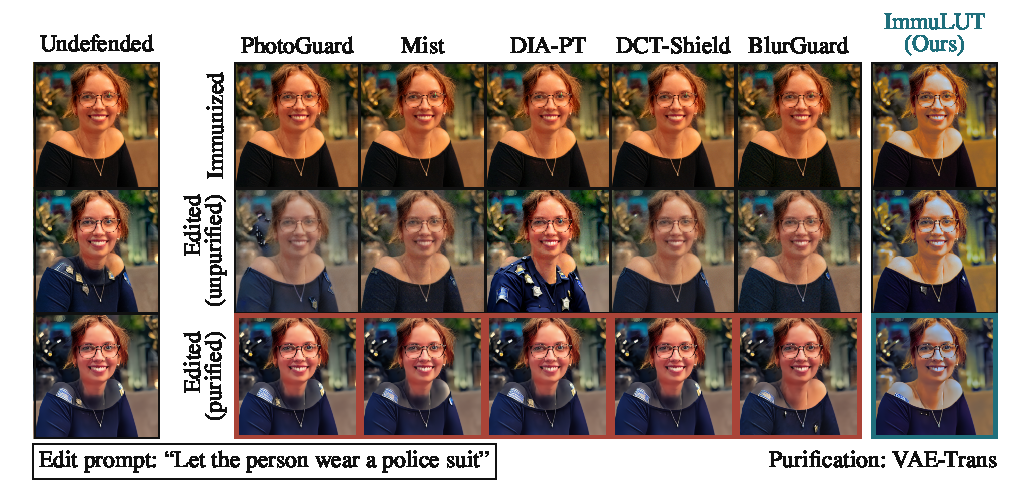
\includegraphics[width=0.85\textwidth]{fig/qualitative_woman_171_police.pdf}
  \caption{Edits with the instruction ``Let the person wear a police suit''. Rows: immunized image, edit without purification, and edit after VAE-Trans. After VAE-Trans, the edits of the additive defenses show epaulettes and a uniform collar, while the edit of \capg{} shows only a small patch on the shoulder. Edit LPIPS after VAE-Trans: .027, .042, .034, .023, .163, and .226.}
  \label{fig:supp_woman_171}
\end{figure*}

\begin{figure*}[t]
  \centering
  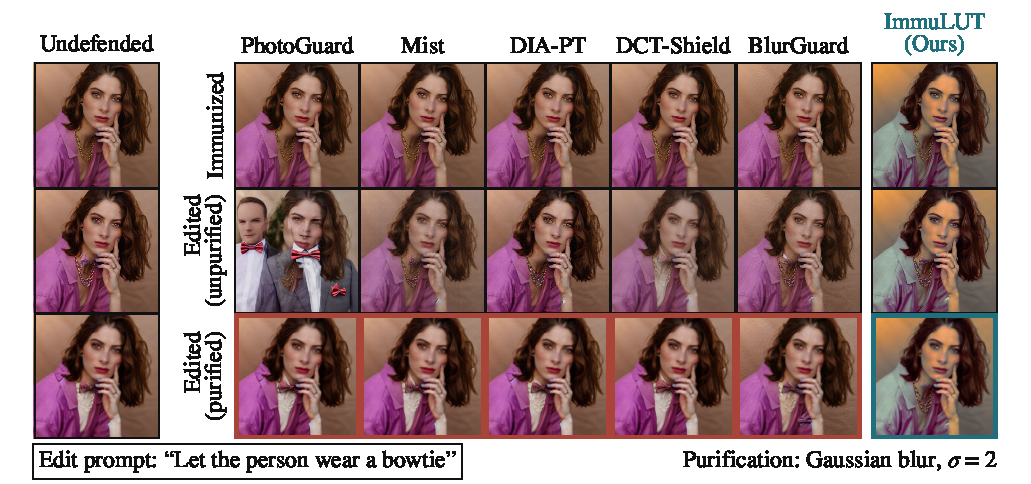
\includegraphics[width=0.85\textwidth]{fig/qualitative_woman_173_bowtie.pdf}
  \caption{Edits with the instruction ``Let the person wear a bowtie''. Rows: immunized image, edit without purification, and edit after Gaussian blur ($\sigma = 2$). After blur, the bowtie appears on the undefended image and on all five additive defenses, but not on \capg{}. Edit LPIPS after blur: .068, .057, .068, .027, .182, and .300.}
  \label{fig:supp_woman_173}
\end{figure*}

\begin{figure*}[t]
  \centering
  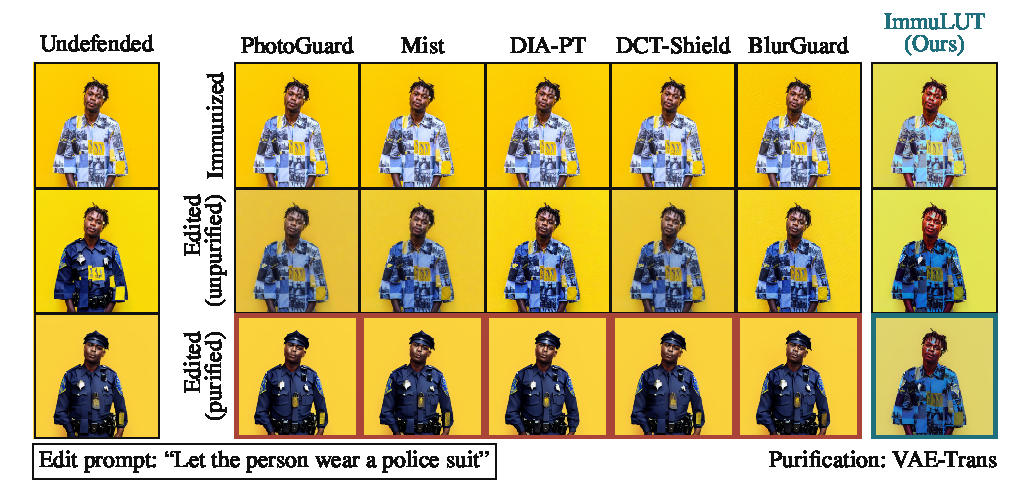
\includegraphics[width=0.85\textwidth]{fig/qualitative_man_91_police.pdf}
  \caption{Edits with the instruction ``Let the person wear a police suit''. Rows: immunized image, edit without purification, and edit after VAE-Trans. After VAE-Trans, the undefended image and all five additive defenses are changed into a complete police uniform, whereas \capg{} keeps the original shirt. Edit LPIPS after VAE-Trans: .055, .031, .077, .036, .062, and .277.}
  \label{fig:supp_man_91}
\end{figure*}
